\renewcommand*{\arraystretch}{1.1}

\subsection*{BI / read / 19}
\label{section:bi-read-19}

\noindent\begin{tabularx}{\queryCardWidth}{|>{\queryPropertyCell}p{\queryPropertyCellWidth}|X|}
	\hline
	query & BI / read / 19 \\ \hline
%
	title & Stranger's interaction
 \\ \hline
%
	pattern & \hfill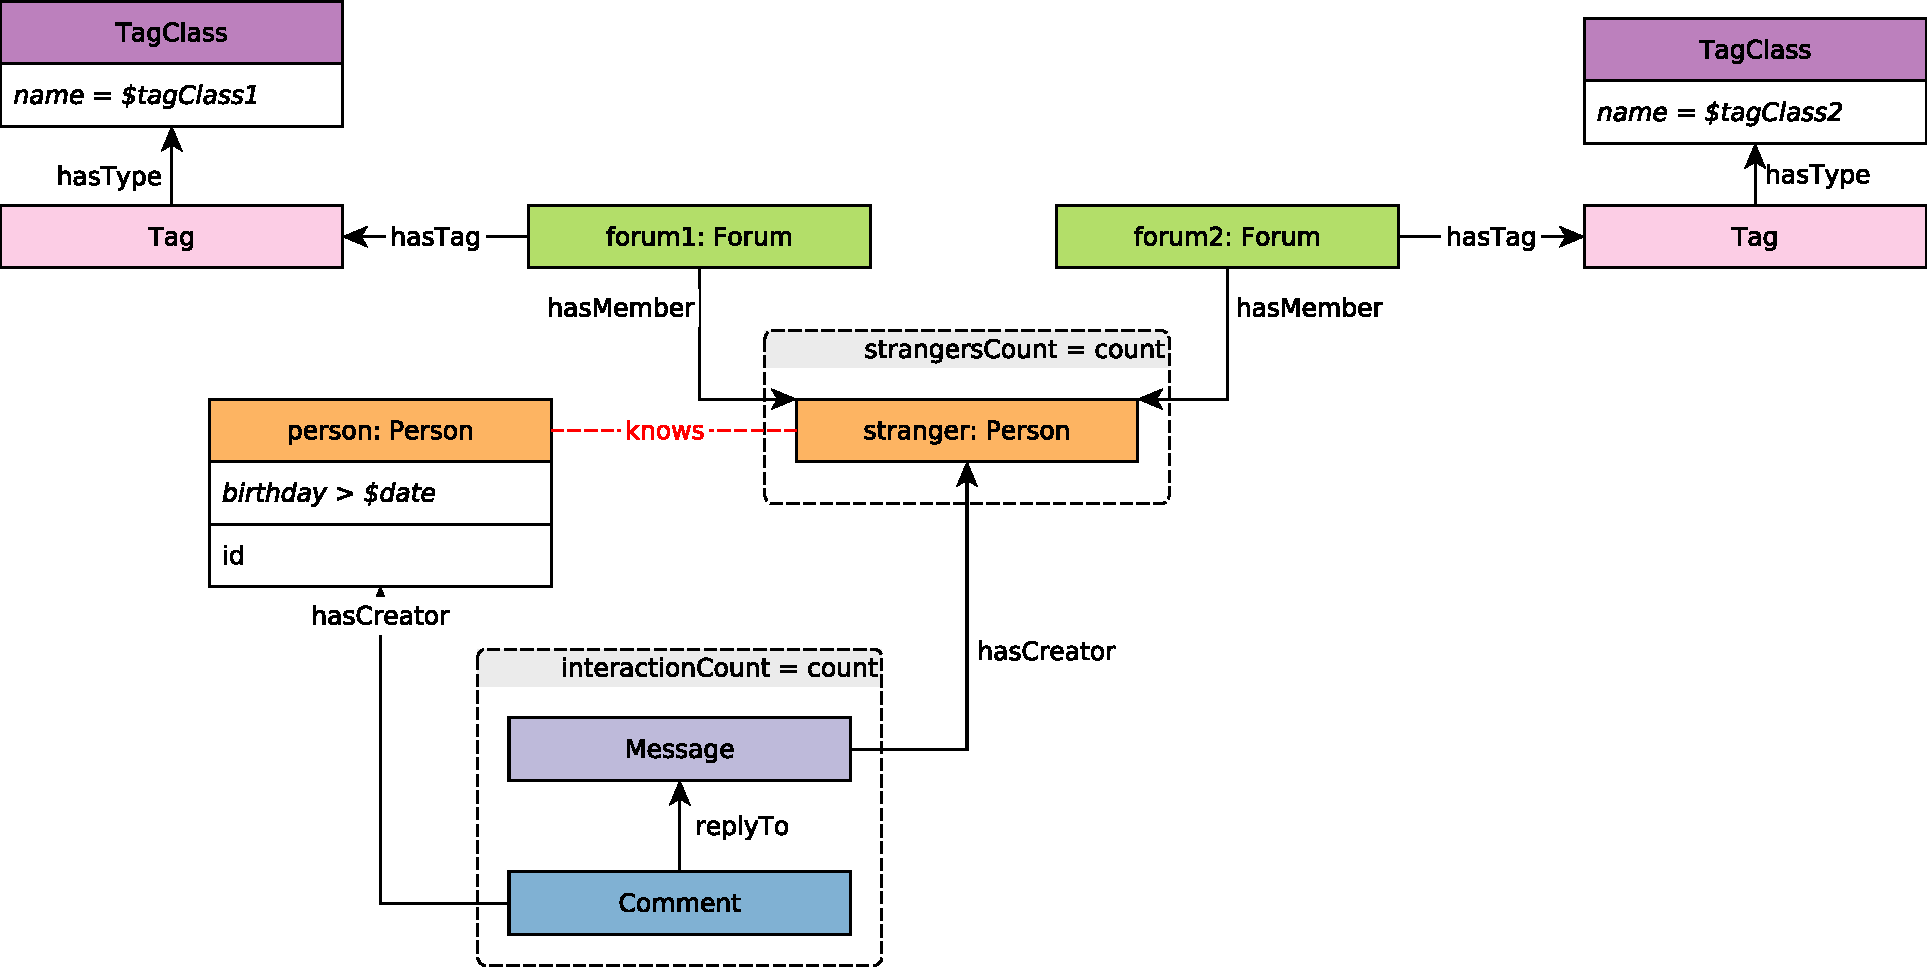
\includegraphics[scale=\patternscale,margin=0cm .2cm]{patterns/bi-read-19}\hfill\vadjust{} \\ \hline
%
	desc. & For all the \emph{Persons} born after a certain \texttt{date}, find all
the strangers they interacted with, where strangers are \emph{Persons}
that do not \emph{know} each other. There is no restriction on the date
that strangers were born.

Consider only strangers that are members of \emph{Forums} tagged with a
\emph{Tag} of \texttt{tagClass1} (direct children not transitive) AND
members of \emph{Forums} tagged with a \emph{Tag} of \texttt{tagClass2}
(direct children not transitive). The tags may be attached to the same
\emph{Forum} or they may not be attached to different \emph{Forums}.

Interaction is defined as follows: if \emph{Person} \emph{A} replies to
a \emph{Message} (\emph{Post} or \emph{Comment}) by another
\emph{Person} \emph{B}, there is an ``interacted with'' relationship
from \emph{A} to \emph{B}. Note that the ``interacted with''
relationship is directed.

For each \emph{Person}, count the number of strangers they interacted
with and total number of times they interacted with them.
 \\ \hline
%
	
		params &
		\innerCardVSpace{\begin{tabularx}{\attributeCardWidth}{|>{\paramNumberCell}c|>{\varNameCell}M|>{\typeCell}m{\typeWidth}|Y|} \hline
		$\mathsf{1}$ & date
 & Date
 &  \\ \hline
		$\mathsf{2}$ & tagClass1
 & String
 &  \\ \hline
		$\mathsf{3}$ & tagClass2
 & String
 &  \\ \hline
		\end{tabularx}}\innerCardVSpace \\ \hline
	
%
	
		result &
		\innerCardVSpace{\begin{tabularx}{\attributeCardWidth}{|>{\resultNumberCell}c|>{\varNameCell}M|>{\typeCell}m{\typeWidth}|>{\resultOriginCell}c|Y|} \hline
		$\mathsf{1}$ & person.id & 64-bit Integer & R &
				 \\ \hline
		$\mathsf{2}$ & strangersCount & 32-bit Integer & A &
				 \\ \hline
		$\mathsf{3}$ & interactionCount & 32-bit Integer & A &
				 \\ \hline
		\end{tabularx}}\innerCardVSpace \\ \hline
	
%
	
		sort		&
		\innerCardVSpace{\begin{tabularx}{\attributeCardWidth}{|>{\sortNumberCell}c|>{\varNameCell}M|>{\directionCell}c|Y|} \hline
		$\mathsf{1}$ & interactionCount
 & $\desc
$ &  \\ \hline
		$\mathsf{2}$ & person.id
 & $\asc
$ &  \\ \hline
		\end{tabularx}}\innerCardVSpace \\ \hline
	%
	limit & 100 \\ \hline
	%
	CPs &
	\multicolumn{1}{>{\raggedright}l|}{
		\chokePoint{1.1}, 
		\chokePoint{1.4}, 
		\chokePoint{2.1}, 
		\chokePoint{2.3}, 
		\chokePoint{2.4}, 
		\chokePoint{3.3}, 
		\chokePoint{5.1}, 
		\chokePoint{7.3}, 
		\chokePoint{7.4}
		} \\ \hline
	%
	%
\end{tabularx}
\queryCardVSpace